\graphicspath{{chapters/greco/images/level5/}}

\subsection{GRECO Level 5 Cuts}
The next stage of cuts, know as the \emph{GRECO Level 5}, or more simply, \emph{L5}, is structured in a similar manner. 
Once again, there exists both a relatively simple cut dedicated to removing accidental triggers due to noise as well as a BDT consisting of six variables.

\subsubsection{L5 Straight Cuts}
The former is a again cut on the number of hits similar to the cleaning applied in the L3 cuts. 
This time, however, a slightly different cleaning is applied, consisting of both a static and a dynamic time window applied to the split DeepCore pulses.
The static window, with a width of 7500 nanoseconds, removes hits that are far from the trigger in order to limit the effect of random detector noise.
The dynamic time window is designed to specifically look for a set of hits spaced very closely in time.
For the L5 noise trigger cut, a dynamic window is chosen of 200 nanoseconds.

After the two time window cleaning algorithms are applied, the resulting hit series is required to posses at least 3 remaining hits to be accepted for further processing.

\subsubsection{Time to 75\% Charge}
\begin{figure}[h]
	\centering
		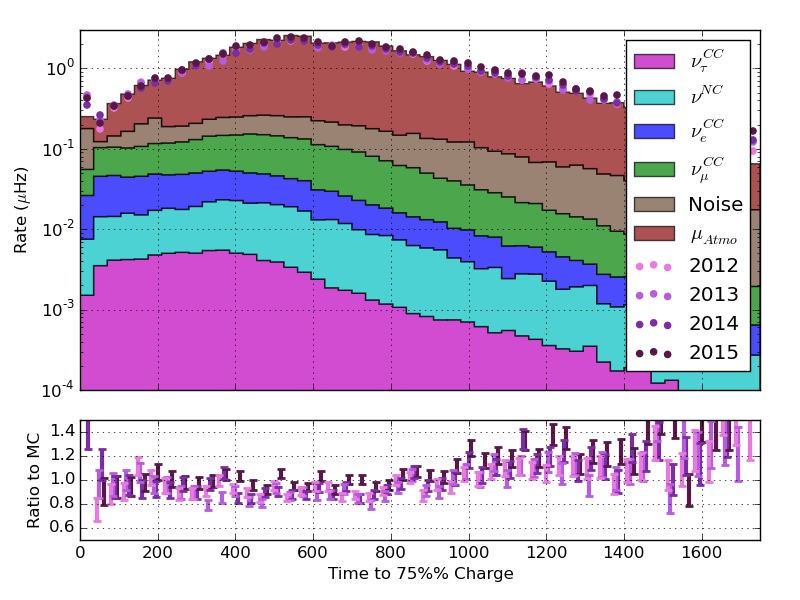
\includegraphics[width=2.5in]{Time_to_75_Charge_log.png}
		\caption[Time to 75\% Charge]{The time to accumulate 75\% of the total charge of the event.}
	\label{fig:time_to_75}
\end{figure}

The first variable used to create the L5 BDT is the amount of time to accumulate 75\% of the total charge, the \emph{$t_{75}$}. 
The idea behind this variable is again similar to that of the QR6 and C2QR6 variables and will not be repeated here.
However, the variable is now produced in the reverse manner: where the QR6 variable refers to the amount of a charge in a given window, the $t_{75}$ instead attempts to find the amount of time for a given charge level, providing an additional handle on the total event length and timing distribution.


\subsubsection{Veto Identified Causal Hits}
\begin{figure}[h]
	\centering
		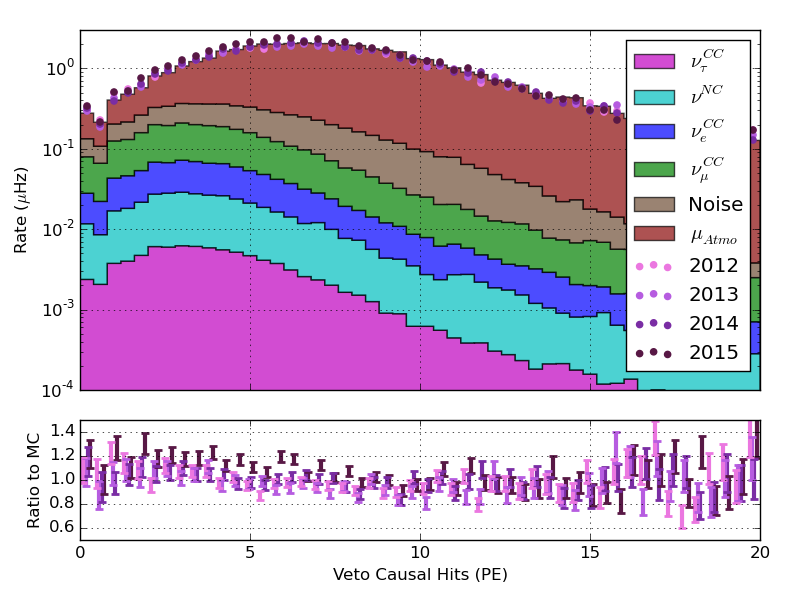
\includegraphics[width=2.5in]{Veto_Causal_Hits_(PE)_log.png}
		\caption[Veto Identified Causal Hits]{The amount of causally-connected charge discovered in the veto region.}
	\label{fig:vich}
\end{figure}

The \emph{Veto Identified Causal Hits} (\emph{VICH}) algorithm is a second choise for the L5 cuts that relies solely on low-level charge information.
In this case, we improve on causality constraints using the trigger time and the position of the first DOM to contribute to the trigger.
The time and distance are calculated to each other hit relative to this simplistic event vertex.
Any hits that occur in a window before the trigger that are approximately causally connected to this hit are recorded, with the total charge thus recorded giving the cut variable.
The window is described in \ref{fig:VICH_definition}


\subsubsection{First Hit $\rho$}
\begin{figure}[h]
	\centering
		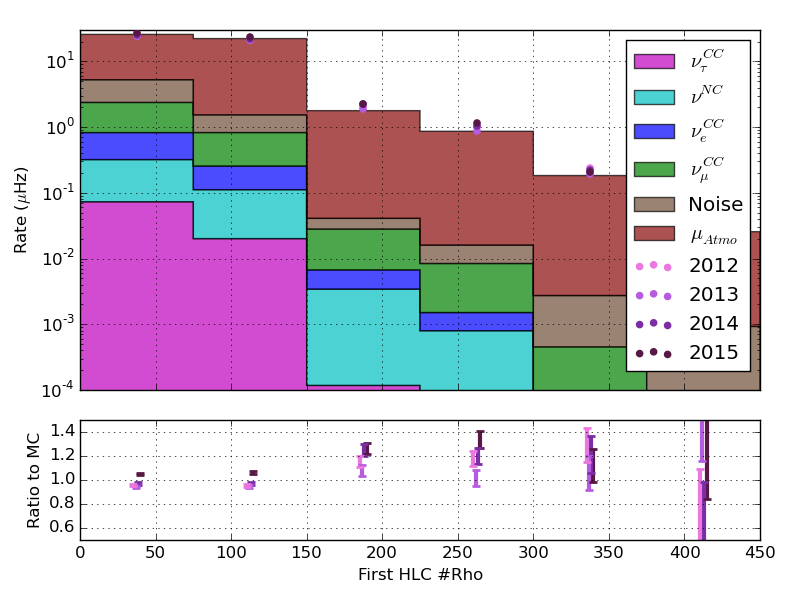
\includegraphics[width=2.5in]{First_HLC_Rho_log.png}
		\caption[First Hit $\rho$ Position]{The radial position of the earliest hit of a cleaned hit series. The radial position is measured relative to string 36, the center of DeepCore.}
	\label{fig:firsthit_rho}
\end{figure}

Further simple event vertices give additional separation power. 
In particular, the radial position of the first hit in a STW cleaned (7500 ns) hit series encompassing solely the DeepCore fiducial volume may be used to identify incoming atmospheric muon events.


\subsubsection{Quartiles CoG}
\begin{figure}[h]
	\centering
		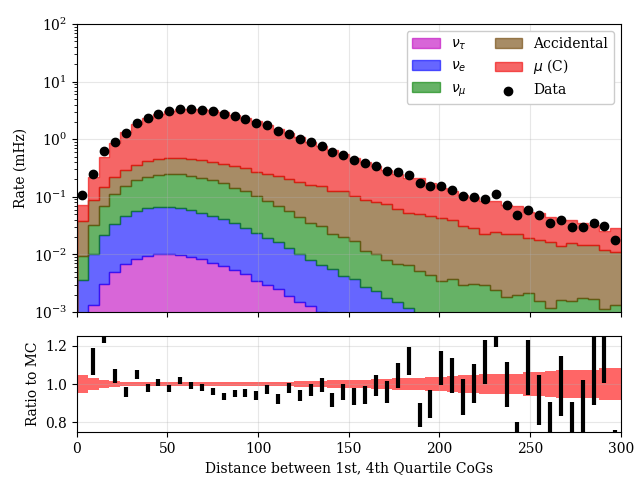
\includegraphics[width=2.5in]{Q1-Q4_Distance_log.png}
		\caption[Quartile Distance]{The distance between the centers of gravity of the first and last quartile in time.}
	\label{fig:quartile_distance}
\end{figure}

The traveling distance of a muon may be exploited in order to identify muons as well.
In particular, a track-like event is expected to travel over a longer distance than a cascade-like event of a similar energy.
Looking at the first and last quartiles in charge, the length of the vector from one of the CoGs to the other can give some simple indiciation of the length of a hypothetical track in the event.

\subsubsection{Z-Travel}
\begin{figure}[h]
	\centering
		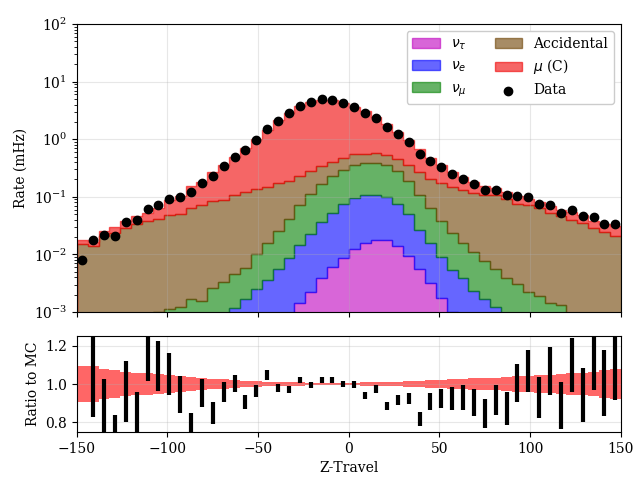
\includegraphics[width=2.5in]{Z-Travel_log.png}
		\caption[Quartile Z-Travel]{The distance traveled in Z between the first and last quartile of hits in time.}
	\label{fig:quartile_ztravel}
\end{figure}

Atmospheric muons are primarily a downgoing feature of the detector, with a flux that approaches zero at the horizon.
Muons will, therefore, leave some information in the depth and directional information collected by the detector.
The first variable to utilize this, \emph{Z-Travel}, identifies the distance in the z-direction between the first and the last quartile of hits using the CoGs calculated in the previous variable.

\subsubsection{SPE Zenith}
\begin{figure}[h]
	\centering
		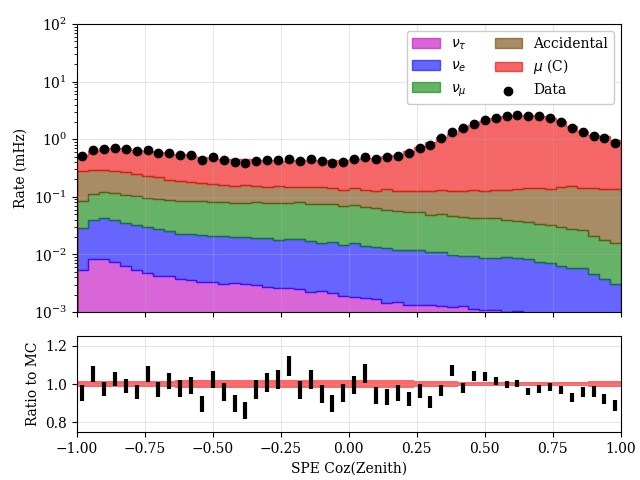
\includegraphics[width=2.5in]{SPE11_Cos(Zenith)_log.png}
		\caption[SPE Reconstruction Zenith Angles]{The zenith angle distribution of events from an 11-iteration SPE fit. The fit assumes an infinite track hypothesis and uses only hit DOMs.}
	\label{fig:spe11_zenith}
\end{figure}

More advanced reconstructions are viable at this level, providing new potential for the identification of atmospheric muons from neutrino candidates.
Using the first pulse on each DOM, a likelihood reconstruction may be produced.
A fast likelihood reconstruction assuming an infinite track passing through the detector with light scattered via the Pandel scattering model of ice is one such tool.

The Pandel model of scattering, while known to be inaccurate, provides an analytic form that is fast to evaluate in order to find the charge expectation as a function of relative position and direction between the hypthesized track and each DOM.
The reconstruction is begins with a seed of some description that my slightly gin-addled mind with no internet access cannot recall.
A total of eleven directions are used as seeds around the seeded position and time, including a seeded direction.
For each hypothesis, the expected charge at different time steps is compared to the observed charge at each DOM using a Poisson binned likelihood.
The best-fit of the eleven reconstructions is returned.

Again, atmospheric muons are primarily downgoing events. 
Therefore the direction of the reconstructed track is a useful tool for separating neutrino signal and atmospheric muon background.


\subsubsection{The L5 BDT}
\begin{figure}[h]
	\centering
		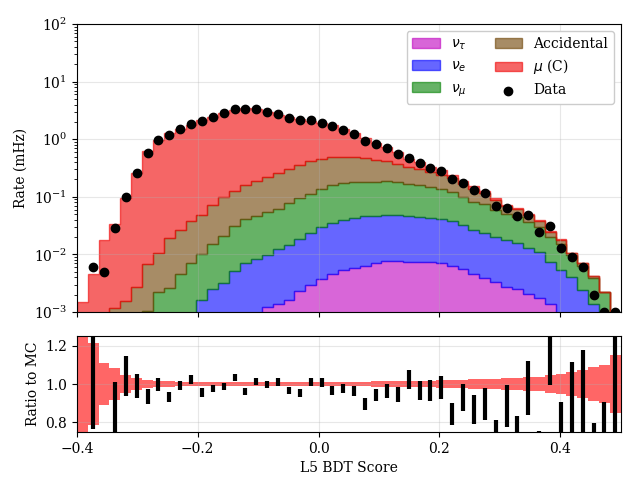
\includegraphics[width=4in]{BDT_Score_log.png}
		\caption[The L5 BDT Score]{The distribution of the boosted decision tree used at L5. A cut is again applied at 0.04 to remove a significant fraction of atmospheric muon background events.}
	\label{fig:L5_bdt_log}
\end{figure}

The six variables described in this section are again used to create a BDT. 
At the time of training, updated versions of both the GENIE and CORSIKA simulations were provided as part of a ongoing upgrade of the IceCube simulation.
In particular, the L5 BDT was trained using simulation files containing the then-newly available Vuvuzela noise model and an updated version of the GENIE Monte Carlo generator.

A set of fifteen variables were tested.
At each step of the training, the least important variable was removed to limit the possible effects of overtraining.
The process continued until changes in the cut efficiency larger than 1\% were observed, resulting in a boost decision tree containing the six most important variables tested as described above.

The distribution of BDT score is shown in \ref{fig:L5BDT_log}. 
The data and simulation show good agreement across the range of scores.
In addition, the distribution of shows some separation from the neutrino events, providing some cut power.

A cut is placed at a score of 0.04, which gives approximately 95\% background rejection with a somewhat significant hit of 30\% to all neutrino rates.




